%%%%%%%%%%%%%%%%%%%%%%%%%%%%%%%%%%%%%%%%%%%%%%%%%%%%%%%%%%%%%%

\documentclass[12pt,ITBthesis]{report}

\usepackage{amsfonts}
\usepackage{amssymb,amsmath}
\usepackage{amsthm}
\usepackage{newlfont}
\usepackage{graphicx}
\usepackage{tabularx}
\usepackage{longtable}
\usepackage{lscape}
%\usepackage{rotating}
\usepackage{latexsym}
\usepackage{natbib}
\usepackage{geometry}
\usepackage{fancyhdr}
\usepackage{xthesis}
\usepackage{xtocinc} %Include Table of Contents as the first entry in TOC
\usepackage{subfigure}
\usepackage{times}
\usepackage[hidelinks]{hyperref}



\bibpunct[, ]{(}{)}{;}{a}{,}{,}


\begin{document}
% \begin{KeepFromToc}
%   \tableofcontents
% \end{KeepFromToc}


%%% this section is responsible for creating bookmarks and cross-links in your pdf document
%\hypersetup{bookmarksnumbered=true, colorlinks=false, bookmarksopen = false, linkcolor=blue ,
%linkbordercolor = 3 3 3, citebordercolor = 3 3 3, urlbordercolor = 3 3 3}


% Fuzz -------------------------------------------------------------------
\hfuzz2pt % Don't bother to report over-full boxes if over-edge is < 2pt
% Line spacing -----------------------------------------------------------

\newlength{\defbaselineskip}
\setlength{\defbaselineskip}{\baselineskip}
\newcommand{\setlinespacing}[1]%
           {\setlength{\baselineskip}{#1 \defbaselineskip}}
\newcommand{\doublespacing}{\setlength{\baselineskip}%
                           {2.0 \defbaselineskip}}
\newcommand{\singlespacing}{\setlength{\baselineskip}{\defbaselineskip}}
% MATH -------------------------------------------------------------------
\newcommand{\A}{{\cal A}}
\newcommand{\h}{{\cal H}}
\newcommand{\s}{{\cal S}}
\newcommand{\W}{{\cal W}}
\newcommand{\BH}{\mathbf B(\cal H)}
\newcommand{\KH}{\cal  K(\cal H)}
\newcommand{\Real}{\mathbb R}
\newcommand{\Complex}{\mathbb C}
\newcommand{\Field}{\mathbb F}
\newcommand{\RPlus}{[0,\infty)}
%
\newcommand{\norm}[1]{\left\Vert#1\right\Vert}
\newcommand{\essnorm}[1]{\norm{#1}_{\text{\rm\normalshape ess}}}
\newcommand{\abs}[1]{\left\vert#1\right\vert}
\newcommand{\set}[1]{\left\{#1\right\}}
\newcommand{\seq}[1]{\left<#1\right>}
\newcommand{\eps}{\varepsilon}
\newcommand{\To}{\longrightarrow}
\newcommand{\RE}{\operatorname{Re}}
\newcommand{\IM}{\operatorname{Im}}
\newcommand{\Poly}{{\cal{P}}(E)}
\newcommand{\EssD}{{\cal{D}}}
% THEOREMS ---------------------------------------------------------------
\theoremstyle{plain}
\newtheorem{thm}{Theorem}[section]

\newtheorem{cor}[thm]{Corollary}
\newtheorem{lem}[thm]{Lemma}
\newtheorem{prop}[thm]{Proposition}
%
\theoremstyle{definition}
\newtheorem{defn}{Definition}[section]
%
\theoremstyle{remark}
\newtheorem{rem}{Remark}[section]
%
\numberwithin{equation}{section}
\renewcommand{\theequation}{\thesection.\arabic{equation}}
%%% ----------------------------------------------------------------------
\setlength{\tclineskip}{1.05\baselineskip}
%%% ----------------------------------------------------------------------

\makeatletter
\renewcommand\listoffigures{%
        \@starttoc{lot}%
}
\makeatother

\makeatletter
\renewcommand\listoftables{%
        \@starttoc{lot}%
}
\makeatother

\makeatletter
\renewcommand\appendix{%
 \par
 \setcounter{chapter}{0}%
 \setcounter{section}{0}%
 \setcounter{subsection}{0}%
 \gdef\thesection{\@Alph\c@section}
 \gdef\@sect##1##2##3##4##5##6[##7]##8{%
  \refstepcounter{##1}%
  \protected@edef\@svsec{\@seccntformat{##1}\relax}%
  \begingroup
    \hspace{-\parindent}##6\appendixname~ {%
    \@hangfrom{\hskip ##3 \relax\@svsec}\par%
    \hspace{-\parindent}\interlinepenalty \@M ##8 \@@par}%
  \endgroup
  \csname ##1mark\endcsname{##7}%
  \addcontentsline{toc}{##1}{\protect\numberline{\csname the##1\endcsname}##7}%
  \@xsect{##5}%
 }%
}%
\makeatother

\setlength{\parskip}{1ex plus 0.5ex minus 0.2ex}


\title{Data Analytics Assessment: Analyse a dataset}

\author{Aaron Ward}

\university{Institute of Technology Blanchardstown }

\dept{School of Informatics and Engineering }

\address{Dublin, Ireland }

%\supervisor{}

\submitdate{2017}

\degree{B.Sc in Computing and Information Technology}


%\dedicate{To my wife\\
% \begin{Huge}{\textbf{Glenda}}\end{Huge}}

%\nobib
%\draft
%\nofront
%\permissionfalse
%\include{ABS}

\setcounter{page}{1} \beforepreface



{ \typeout{Abbreviations}
% Thesis Abbreviation ------------------------------------------------------

\prefacesection{Abbreviations}


%%%%%%%%%%%%%%%%%%%%%%%%%%%%%%%%%%%%%%%%%%%%%%%%%%%%%%%%%%%%%%%%%%%%%%%%%%%%%%%%
% Create a list of all abbreviations that you've used throughout your thesis.  %
% Order the abbreviations in alphabetical order                                %
%%%%%%%%%%%%%%%%%%%%%%%%%%%%%%%%%%%%%%%%%%%%%%%%%%%%%%%%%%%%%%%%%%%%%%%%%%%%%%%%

\begin{longtable}{p{90pt}l}
\hline ANN    	&\vline  Artificial Neural Network \\
\hline CNN      &\vline  Convultional Neural Network \\
\hline ReLU     &\vline  Rectified Linear Unit \\
\hline 
\
\end{longtable}






% ----------------------------------------------------------------------
 %write your list of abbreviations in a file called abbreviations.tex
}

%{ \typeout{Glossary}
%\include{glossary}
%}



% ------------------------------------------------------------------------
\afterpreface
\def\baselinestretch{1}
\setlinespacing{1.66}
% ------------------------------------------------------------------------

\pagestyle{fancy}
% \renewcommand{\chaptermark}[1]% 
%{\markboth{\MakeUppercase{\thechapter.\ #1}}{}}
% \renewcommand{\sectionmark}[1]%
%{\markright{\MakeUppercase{\thesection.\ #1}}}
\renewcommand{\headrulewidth}{0.5pt}
\renewcommand{\footrulewidth}{0pt}
\newcommand{\helv}
{%
\fontfamily{bch}\fontseries{b}\fontsize{9}{11}\selectfont} \fancyhf{} \fancyhead[LE,RO]{\helv \thepage}
\fancyhead[LO]{\helv \rightmark} \fancyhead[RE]{\helv \leftmark}

% ------------------------------------------------------------------------
\setlinespacing{1.0}


\prefacesection{Text Analytics Using Rapid Miner}

\section*{Business Understanding}

This following sections shall describe the business objectives, the mining objectives, a analysis and plan for the proposed project.

\subsection*{Business Objective}
The objective of this project is to mine unstructured data using Rapid Miner.

\subsection*{Data Mining objective}
\begin{itemize}
	\item The main objective is to mine articles about Machine Learning, Deep Learning and Robotics. 
	\item Web crawling will be implemented to find related text on the topics.
	\item Preprocessing steps shall be put in place in order to produce the most predictive words for modeling.
	\item Multiple clustering and classification models will be used to identify the texts.
\end{itemize}

\subsection*{Project analysis}
% (cost benifit analysis; risk assessment; resouces needed; assumptions)
In terms of a cost benefit analysis, this project deems relatively efficient due to the benefits out weighing the costs. The proposed assignment poses minimal risk as only a few events may delay the production of the project, such as unavailable texts and misclassification, which are very unlikely. The resources required for this project include: The RapidMiner software and all it's operators related to the data mining objective, articles from online resources, 13 documents based on 3 categories and a online word cloud service for visualisation of predictive words or phrases. 

 
\subsection*{Project plan}
There are a number of steps taken in relation to this project.
\begin{itemize}
	\item Initially, Three categories are decided on. Two topics should be relatively similar, and the last on will be unrelated. In this case, they are based on Deep Learning, Machine Learning and robitics.
	\item Thirteen texts are sourced online for each category. Ten shall be used for training datasets and three shall be used for testing. Web crawling will be implemented using RapidMiner for three of those texts. The steps taken will be documented 
	\item These source articles will be downloaded into their respective folders based on their class label.
	\item A word cloud will be creating to visualise the frequently occurring terms.
	\item Preprocessing steps shall be experimented with to compare stemmers, determine which words are predominantly more predictive, apply pruning and comparing accuracy based on different vectors and documenting the results.
	\item Apply two algorithms for clustering and classification and discuss the accuracy of them.
	\item Lastly, an evaluation of the project will be performed, which will assess the overall result in relation with the business objectives. 
\end{itemize}

%%%%%%%%%%%%%%%%%%%%%%%%%%%%%%%%%%%%%%%%%%%%%%%%%%%%%%%%%%%%

\section*{Data Understanding}
%Eliminate common words & stop words
%Eliminate rare words
%Identify phrases

As previously mentioned, thirteen texts have been obtain online according to three categories: machine learning, deep learning and robotics.
In order to obtain a better insight to the commonly occurring word in the files of each category, word clouds were made. As seen in Figure \ref{mlfig}, Figure \ref{dlfig} and Figure \ref{robfig} three word images were made to visualise the frequent terms. The larger the word appears in the image, the more often it appears in the documents that have been collected.
For machine learning, it is clear that the terms \textbf{knn}, \textbf{training}, \textbf{decision tree}, \textbf{naive bayes} and \textbf{classification}.

\begin{figure}[ht]
	\begin{center}
		\advance\leftskip-3cm
		\advance\rightskip-3cm
		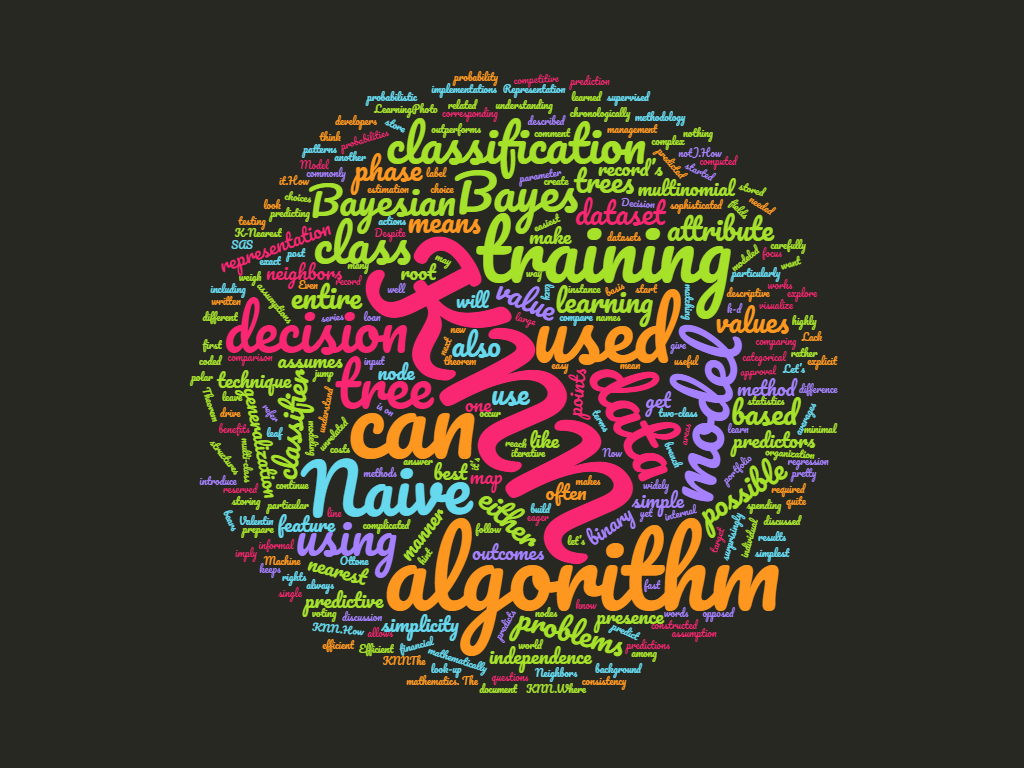
\includegraphics[keepaspectratio=true,scale=0.4]{__resources/machine_learning.png}
		\caption{Word cloud for the machine learning category}
		\label{mlfig}
	\end{center}
\end{figure}

\newpage

A more concise description of deep learning can be seen in Figure 2. Although the two categories are related, these terms seem to focus more so on words like \textbf{networks}, \textbf{neural}, \textbf{CNN's}, \textbf{model} and \textbf{recurrent} to name a few.

\begin{figure}[ht]
	\begin{center}
		\advance\leftskip-3cm
		\advance\rightskip-3cm
		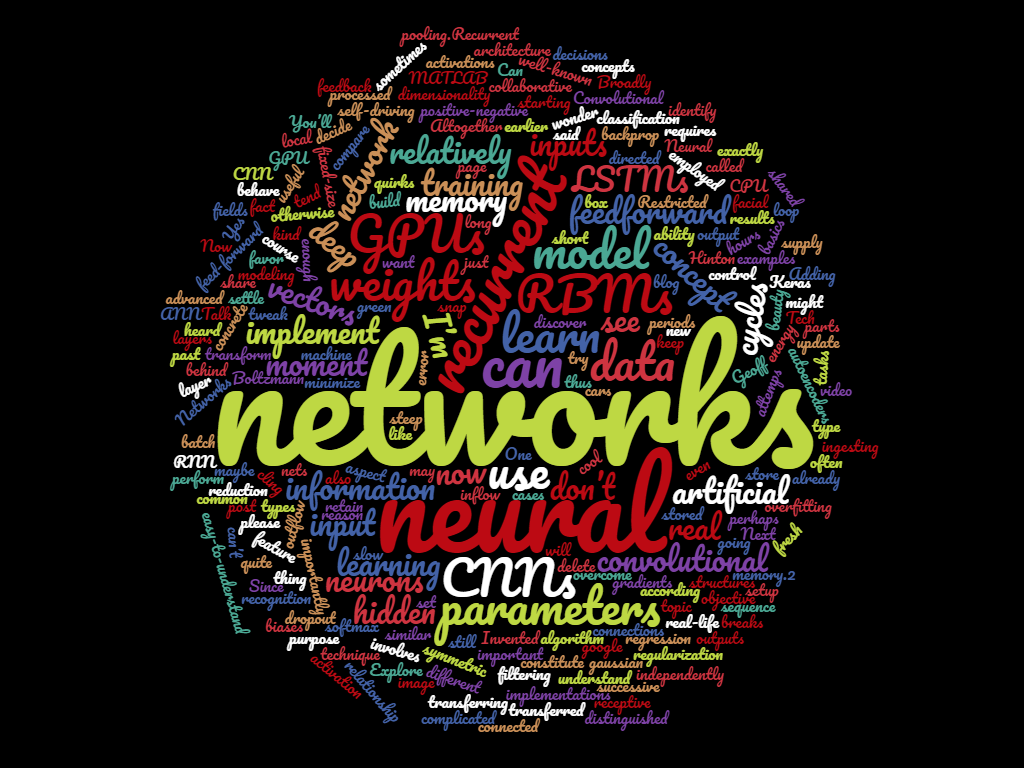
\includegraphics[keepaspectratio=true,scale=0.4]{__resources/deep_learning.png}
		\caption{Word cloud for the deep learning category}
		\label{dlfig}
	\end{center}
\end{figure}

Lastly, we see the terms generated for the robotics category. Evidently, these words are not related to machine learning or deep learning as they share very few words to the documents in the other two categories. The prominent words found here are \textbf{robots}, \textbf{humans} or \textbf{humanoid} and  \textbf{robotics}

\newpage


\begin{figure}[ht]
	\begin{center}
		\advance\leftskip-3cm
		\advance\rightskip-3cm
		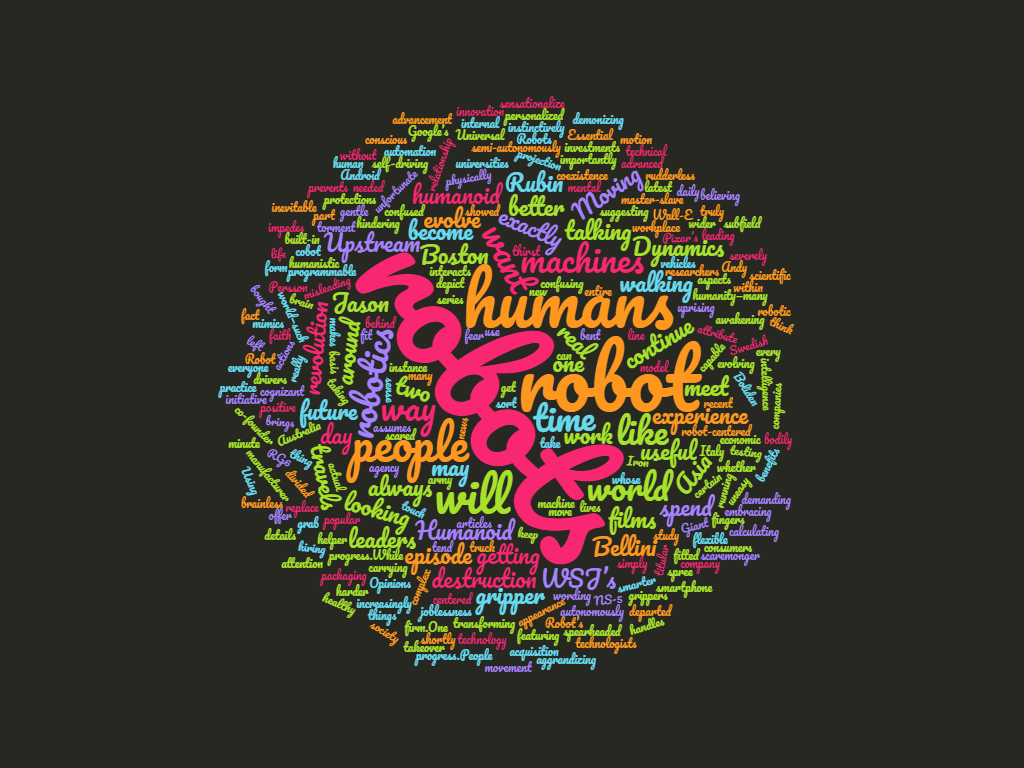
\includegraphics[keepaspectratio=true,scale=0.4]{__resources/robotics.png}
		\caption{Word cloud for the robotics category}
		\label{robfig}
	\end{center}
\end{figure}


Not only do these word clouds help determine predictive words, but also provide certain words that are not useful for the mining objects,also known as stop words. Certain stop words in these figures are "I'm", "thing",  "makes" for example. These words can be ambiguous depending on the sentiment of the article being read or just common English phrases, therefore they should not be included in the working model. \\
Furthermore, potential synonyms can be found in these word clouds. To reduce dimensionality, it is beneficial to specify words that may hold the same meaning. For instance, it can be seen that in the category of robotics, the terms "robot" and "robotics" are in interchangeable, therefore they can be classes as synonyms of one another. Another example of this could be the phase "neural network" and "ANN", which the latter is a acronym for "neural network" therefore that can also be classed as a synonym.

\newpage

%%%%%%%%%%%%%%%%%%%%%%%%%%%%%%%%%%%%%%%%%%%%%%%%%%%%%%%%%%%%
\newpage
\section*{Data Preparation}



%Generate a document vector based on
%selected concepts (terms and phrases)


%%%%%%%%%%%%%%%%%%%%%%%%%%%%%%%%%%%%%%%%%%%%%%%%%%%%%%%%%%%%
\section*{Modeling}

\subsection*{Modeling techniques}
\subsubsection*{Clustering}

\subsubsection*{Classification}

\subsection*{Test Design}
%e.g. split documents into training set and test set

\subsection*{Build and Assess the Model}

%%%%%%%%%%%%%%%%%%%%%%%%%%%%%%%%%%%%%%%%%%%%%%%%%%%%%%%%%%%%

\section*{Evaluation}
%Assessment of data mining reults with
%respect to original business objectives

%%%%%%%%%%%%%%%%%%%%%%%%%%%%%%%%%%%%%%%%%%%%%%%%%%%%%%%%%%%%
\subsection*{Project review}

\subsection*{Project deployment}
%Generate document vectors for new
%documents, and run the model.



\prefacesection{Assignment}


The initial steps of implementing a fuzzy logic system are as follows:
\begin{itemize}
	\item Crisp inputs are converted to set of fuzzy linguistic variable, linguistic terms and membership functions in what is known as fuzzification. 
	\item Based on a set of rules, an inference is made
	\item Lastly, defuzzification is implemented by using the membership functions to provide crisp results.
\end{itemize}
Linguistic variables are natural language values assigned to ranges of numeric inputs or outputs. These linguistic variables can have a set of real life terms to used to define a portion of the overall variable. For example, the linguistic variable \textbf{height} may have the terms {short, medium or tall etc.}. 

\section*{Linguistic Variables}
Based on the requirements of the system, linguistic variables need to be defined for the fuzzy logic system. We know that there are two input variables: "Level" and "Demand". Additionally, an output variable is specified to represent the command given to the pumping system, which will be defuzzified to a final crisp output. Each of these variables should be segmented into the appropriate terms. 
\subsection*{Level}
With this variable, five terms have been used to define the ranges of the level in the water. The terms are as follows: 
\textbf{Level(l) = {very\_low, low, average, high, very\_high}.}\\
The membership functions are based on the ranges specified in the assignment document. Level of the water in the tank can range from between 0 and 100. The type of membership functions used are trapezoidal and triangle. The trapezoidal function are used on the most extreme cases such as very\_low and very\_high and triangle are used on the low, average and high. See figure \ref{member1} for graphical representation.

\begin{figure}[ht]
	\begin{center}
		\advance\leftskip-3cm
		\advance\rightskip-3cm
		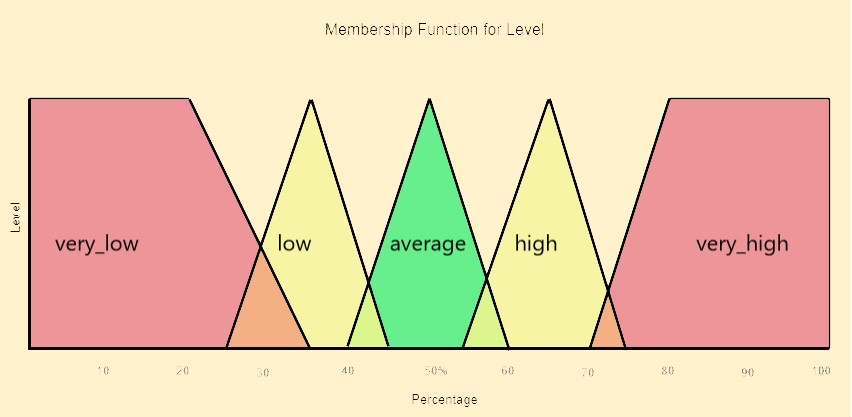
\includegraphics[keepaspectratio=true,scale=0.6]{__resources/level.jpg}
		\caption{Membership functions for Level}
		\label{member1}
	\end{center}
\end{figure}

\subsection*{Demand}
Like the level variable, five linguistic terms were made. The terms are as follows: \textbf{demand(d) = {very\_low, low, middle, high, very\_high}}. The demand variable has a range of -1 and 1.5. The same structure of two trapezoids and three triangle functions were used. 

\begin{figure}[ht]
	\begin{center}
		\advance\leftskip-3cm
		\advance\rightskip-3cm
		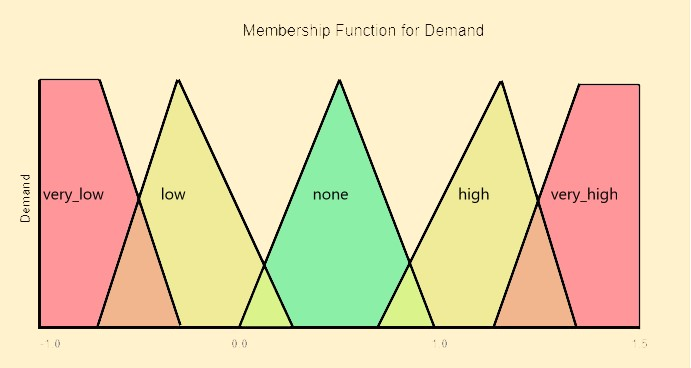
\includegraphics[keepaspectratio=true,scale=0.6]{__resources/demand.jpg}
		\caption{Membership functions for demand}
		\label{member2}
	\end{center}
\end{figure}


\newpage

\section*{Rule Terms}
in order to establish an output variable a set of rules must be defined control the value of the output variable. The three terms used for the output variable are as follows: \textbf{Command = {pump\_in, no\_pump, pump\_pump out}}. The following diagram shows the membership functions of the output variable command.
\begin{figure}[ht]
	\begin{center}
		\advance\leftskip-3cm
		\advance\rightskip-3cm
		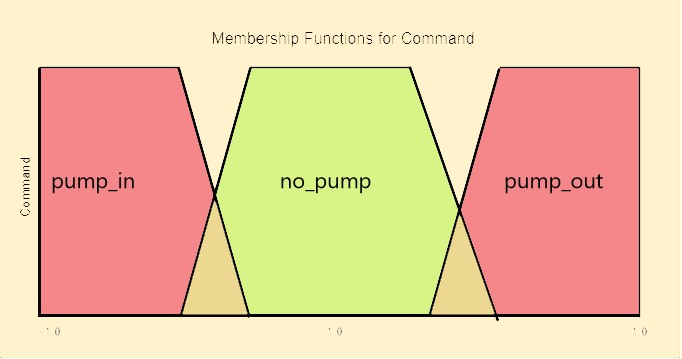
\includegraphics[keepaspectratio=true,scale=0.6]{__resources/command.jpg}
		\caption{Membership functions for command}
		\label{member2}
	\end{center}
\end{figure}
\newpage
A rule matrix will be utilized to illustrate the number of possible rules in the system. The top row signifies the demand variable with the terms it has been provided. Also, the first column displays the Level linguistic variable and it's terms. The intersection terms in the cells contain the command output variable that will be used to control the system.\\

\begin{tabular}{|c|c|c|c|c|c|}
	\hline 
	& \multicolumn{5}{c|}{\textbf{Demand}} \\ 
	\hline 
	\textbf{Level} & very\_low & low & middle & high & very\_high \\ 
	\hline 
	very\_low & pump\_in & pump\_in & pump\_in & pump\_in & no\_pump \\ 
	\hline 
	low & pump\_in & pump\_in & no\_pump & pump\_out & no\_pump \\ 
	\hline 
	average & no\_pump & no\_pump & no\_pump & pump\_out & pump\_out \\ 
	\hline 
	high & no\_pump & pump\_out & pump\_out & pump\_out & pump\_out \\ 
	\hline 
	very\_high & pump\_out & pump\_out & pump\_out & pump\_out & pump\_out \\ 
	\hline 
\end{tabular} \\\\
Following the implementation of the rule matrix, a set of some the possible rules that could be used in the system need to be defined using an \textit{IF-THEN} format. 


 \begin{longtable}{|l|>{\raggedleft\arraybackslash}p{4cm}|l|l|l}
	\hline 
 	\multicolumn{4}{|l|}{IF (level is very\_low) and (demand is very\_low or low or middle or high) THEN command is pump\_in} \\ 
 	\hline 
 	\multicolumn{4}{|l|}{IF (level is very\_low) and (demand is very\_high) THEN command is no\_pump} \\ 
 	\hline 
 	\multicolumn{4}{|l|}{IF (level is low) and (demand is very\_low or low) THEN command is pump\_in} \\ 
 	\hline 
 	\multicolumn{4}{|l|}{IF (level is low) and (demand is high or very\_high) THEN command is pump\_out} \\ 
 	\hline 
 	\multicolumn{4}{|l|}{IF (level is average) and (demand is very\_low or low or middle) THEN command is no\_pump} \\ 
 	\hline 
 	\multicolumn{4}{|l|}{IF (level is average) and (demand is high or very\_high) THEN command is pump\_out} \\ 
 	\hline 
 	\multicolumn{4}{|l|}{IF (level is high) and (demand is very\_low) THEN command is no\_pump} \\ 
 	\hline 
 	\multicolumn{4}{|l|}{IF (level is high) and (demand is low or middle or high or very\_high) THEN command is pump\_out} \\ 
 	\hline 
 	\multicolumn{4}{|l|}{IF (level is very\_high) and (demand is very\_low or low or middle THEN command is pump\_out} \\ 
 	\hline
 	\multicolumn{4}{|l|}{IF (level is very\_high) and (demand is high or very\_high) THEN command is pump\_out} \\ 
 	\hline 
 \end{longtable}

After some experimentation with the rules, it appeared that the more rules that were applied, and the more complex the rules were, the worse the system performed. Therefore, only five of the rules where kept in the final implementation. Using the check boxes, the controller maintains the level of water in the tank between the 40\% and 70\% requirement.



\section*{Conclusion}
In conclusion, this report laid out the purpose of this project, explained the linguistic variables and the terms used within those variable. Membership functions where illustrated for each variable and specified the rules used within the program to keep the controller at a state between the 40\% and 70\% requirements.  


\end{document}
% ------------------------------------------------------------------------
%%%      \setlength\LTleft{1pt}
